\chapter*{Problema C - Caminos y más Caminos}

%\begin{center}
%  \begin{tabular}{ | l | l | l | }
%    \hline
%    Tiepo Límite: 2u & Memoria Límite: 512mb & Código Fuente: %\texttt{cupolimitado.\{java|cpp|c|py\}} \\
%    \hline
%  \end{tabular}
%\end{center}

Schnitzel es una hámster muy inteligente y con mucho tiempo libre. Hace apenas unos días se mudó a un nuevo hogar que aún no termina de explorar, sin, embargo, sabe que en él hay dos ruedas (A y B) entre las cuales hay un camino que aún desconoce; también sabe que los pasillos de su nuevo hogar tienen la forma de una cuadrícula de $m \times n$, como se muestra en la siguiente figura.

\begin{center}
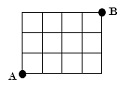
\includegraphics{Cuadricula}
\end{center}

A Schnitzel le gustaría conocer su hogar en su totalidad, así que quiere recorrer todos los posibles caminos que hay para llegar de la primera a la segunda rueda. Tu misión es ayudar a Schnitzel a calcular el tiempo que le tomaría pasar por todos los caminos posibles de su nuevo hogar siguiendo las siguientes reglas:

\begin{itemize}
    \item Schnitzel siempre comienza su exploración en la rueda A.
    \item Recorrer el lado de una celda cualesquiera le toma $t$ segundos.
    \item Únicamente puede avanzar hacia la derecha y hacia arriba.
    \item Una vez que llegue a la segunda rueda, Schnitzel volverá a la primera por el camino que ella desee, y  dado que este punto no cumple con la regla anterior, este camino no deberá ser considerado como uno más, así como el tiempo que tarde en hacerlo no deberá ser sumado a la duración de su paseo.
\end{itemize}


\subsection*{Entrada}

La primera línea será únicamente un entero positivo $C$, tal que $0 < C \leq 100$, el número de casos que vienen a continuación, seguido de $C$ líneas (una para cada caso). En cada línea se dan tres enteros positivos separados por un espacio $m$, $n$ y $t$.


\subsection*{Salida}

Para cada caso, imprime en una línea distinta el tiempo (en segundos) que le tome a Schnitzel recorrer todos los caminos distintos de la rueda A a la rueda B.


\subsection*{Límites de los conjuntos de datos}

\begin{itemize}
\item Pequeño: $1 \leq m+n \leq 10$, $1 \leq t \leq 50$ $\quad \quad \quad \;\;$ $40$ puntos.
\item Mediano: $1 \leq m+n \leq 15$, $1 \leq t \leq 100$ $\quad \quad \quad$ $20$ puntos.
\item Grande: $\,\; 1 \leq m+n \leq 50$, $1 \leq t \leq 100$ $\quad \quad \quad$ $40$ puntos.
\end{itemize}

\begin{multicols}{2}
\subsection*{Entrada Ejemplo}
\begin{verbatim}
3
3 4 1
2 3 3
4 6 50
\end{verbatim}
\columnbreak
\subsection*{Salida Ejemplo}
\begin{verbatim}
245
150
105000
\end{verbatim}
\end{multicols}

